\documentclass{beamer}
%\usetheme{boxed}

\usepackage{ae}
\usepackage{lmodern}

\definecolor{nesrocolor}{RGB}{200,200,255}
\setbeamertemplate{background canvas}[vertical shading][bottom=white,top=nesrocolor]

\setbeamercolor{structure}{fg=black}
\setbeamercolor{title}{fg=black}
\setbeamercolor{titlelike}{fg=black}
\setbeamercolor{section in sidebar}{fg=black}
\setbeamercolor{section in sidebar shaded}{fg=black}

\useinnertheme{default}


\newcommand{\backupbegin}{
   \newcounter{finalframe}
   \setcounter{finalframe}{\value{framenumber}}
}
\newcommand{\backupend}{
   \setcounter{framenumber}{\value{finalframe}}
}


\setbeamertemplate{footline}
{
  \leavevmode
  \hbox{
  \begin{beamercolorbox}[wd=1.0\paperwidth,ht=2.25ex,dp=2ex,center]{author in head/foot}%
    %\usebeamerfont{author in head/foot} Tomas Nesrovnal, FIT CVUT
Tom{\'{a}}\v{s} Nesrovnal $|$ Comma-shell, interaktivn{\'{i}} debugger shellu $|$ \insertframenumber{} / \inserttotalframenumber\hspace*{2ex}
  \end{beamercolorbox}
  }
  \vskip0pt%
}
\makeatother

%gets rid of some non important things
\setbeamertemplate{navigation symbols}{}
\setbeamercolor{separation line}{}

\usepackage{ucs}
\usepackage[utf8x]{inputenc}
\usepackage[czech]{babel}
\usepackage{palatino}
\usepackage{graphicx}

\author{Tomáš Nesrovnal}
\title{Comma-shell, interaktivní debugger shellu}
\institute{Fakulta informačních technologií\\České vysoké učení technické v Praze\\Obor: Systémové programování\\Vedoucí práce: Ing.~Jan Baier}

\begin{document}

%%%%%%%%%%%%%%%%%%%%%%%%%%%%%%%%%%%%%%%%%%%%%%%%%%%%%%%%%%%%%%%%%%%%%%%%%%%%%%%%

\frame{
\titlepage
}

\frame{
	\begin{exampleblock}{Zadání práce	}
		\begin{itemize}
			\item Proveďte rešerši existujících nástrojů pro statickou analýzu, krokování a hledání chyb v BASH skriptech.
			\item Navrhněte a implementujte nástroj, který umožní psát uživatelské skripty pro analýzu příkazů a ovlivňování jejich spouštění a vykonávání. Nástroj musí umožňovat krokovat složitější skripty po jednotlivých příkazech. Pro analýzu spouštěných skriptů využijte vhodný nástroj z rešeršní části.
			\item Vytvořte ukázkové skripty pro zvrácení, či zamezení efektů základních příkazů z GNU coreutils. Zaznamenávejte jejich spouštění a umožněte jimi provedené změny vrátit do původního stavu.
		\end{itemize}
	\end{exampleblock}
}

%%%%%%%%%%%%%%%%%%%%%%%%%%%%%%%%%%%%%%%%%%%%%%%%%%%%%%%%%%%%%%%%%%%%%%%%%%%%%%%%

%\section*{Obsah - }
%\frame{
%	\frametitle{Obsah prezentace FIXME: chci vubec obsah?}
%	\tableofcontents
%}

%%%%%%%%%%%%%%%%%%%%%%%%%%%%%%%%%%%%%%%%%%%%%%%%%%%%%%%%%%%%%%%%%%%%%%%%%%%%%%%%	

%\section{}

%%%%%%%%%%%%%%%%%%%%%%%%%%%%%%%%%%%%%%%%%%%%%%%%%%%%%%%%%%%%%%%%%%%%%%%%%%%%%%%%	

\section{Cíl práce}
\begin{frame}
	\frametitle{Cíl práce}
	\begin{itemize}
		\item Vytvořit nástroj usnadňující výuku v shellu Bash
		\item Analýza příkazů před jejich spuštěním
		\item Jednoduchý, interaktivní debugger příkazů v příkazové řádce
		\item Sada bezpečných příkazů
	\end{itemize}
\end{frame}

\section{Existující řešení}
\begin{frame}
	\frametitle{Existující řešení}
	\begin{itemize}
		\item Debugování skriptů: Bash Debugger (podobné GNU GDB)
		\item Statická analýza skriptů: ShellCheck
	\end{itemize}
\end{frame}

%\subsection{Bash Debugger}
%\begin{frame}
%	\frametitle{Existující řešení: Bash Debugger}
%	\begin{exampleblock}{Výhody}
%		\begin{itemize}
%			\item Ovládání jako GNU GDB
%		\end{itemize}
%	\end{exampleblock}
%	\begin{alertblock}{Nevýhody}
%		\begin{itemize}
%			\item Pouze pro skripty
%		\end{itemize}
%	\end{alertblock}
%	
%		
%\end{frame}
%\begin{frame}
%	\frametitle{Existující řešení: Bash Debugger}
%	\begin{figure}
%		\centering
%		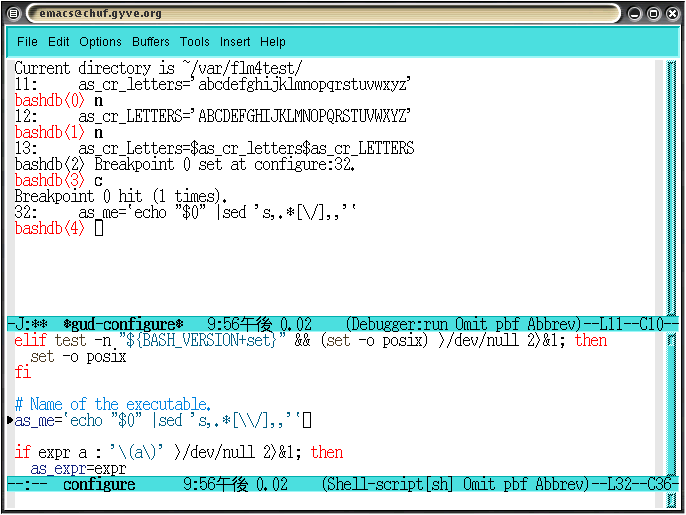
\includegraphics[width=1.0\textwidth]{./images/bashdb-break_invert}
%		%\caption{Bash Debugger}
%	\end{figure}	
%\end{frame}
%
%
%\subsection{ShellCheck}
%\begin{frame}
%	\frametitle{Existující řešení: ShellCheck}
%	\begin{exampleblock}{Výhody}
%		\begin{itemize}
%			\item Databáze "špatného kódu"
%		\end{itemize}
%	\end{exampleblock}
%	\begin{alertblock}{Nevýhody}
%		\begin{itemize}
%			\item Napsaný v jazyce Haskell
%			\item Pouze pro skripty
%		\end{itemize}
%	\end{alertblock}
%\end{frame}

%%%%%%%%%%%%%%%%%%%%%%%%%%%%%%%%%%%%%%%%%%%%%%%%%%%%%%%%%%%%%%%%%%%%%%%%%%%%%%%%

\section{Comma-shell}

%%==============================================================================

\subsection{Hooks}
\begin{frame}
	\frametitle{Comma-shell: Hooks}
	
	\begin{exampleblock}{Využití}
		\begin{itemize}
			\item Framework pro vytváření uživatelských skriptů
			\item Spouštění skriptů před vykonáním příkazů z příkazové řádky
			\item Příkazy k vykonání je možné měnit, nebo nevykonávat
		\end{itemize}
	\end{exampleblock}	
	
	\begin{exampleblock}{Implementace}
		\begin{itemize}
			\item Zastavení všech příkazů pomocí DEBUG trap v módu extdebug
			\item Příkaz k vykonání se zjišťuje pomocí příkazu history
			\item Vykonávání příkazů probíhá pomocí příkazu eval
			\item Hook dostává v parametru příkaz a identifikátor
		\end{itemize}
	\end{exampleblock}
\end{frame}


\begin{frame}
	\frametitle{Ukázkya: ShellCheck Hook}
	\begin{figure}
		\centering
		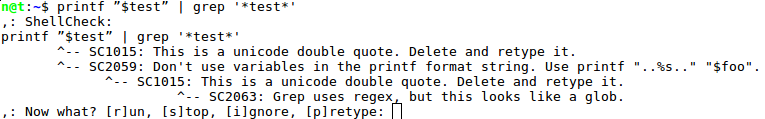
\includegraphics[width=1.0\textwidth]{./images/shellcheck}
		%\caption{Bash Debugger}
	\end{figure}	
\end{frame}



\subsection{Debugger}
\begin{frame}
	\frametitle{Comma-shell: Debugger}
	
	\begin{exampleblock}{Využití}
		\begin{itemize}
			\item Spouštění částí příkazů v příkazové řádce
		\end{itemize}
	\end{exampleblock}		
	
	
	\begin{exampleblock}{Implementace}
		\begin{itemize}
			\item Jedná se o hook, původní příkaz se nevykoná
			\item Pomocí knihovny bashlex se prochází AST příkazu
			\item K částem příkazu se přidá další kód a v Bashi je vykonán pomocí příkazu eval 
		\end{itemize}
	\end{exampleblock}		
\end{frame}

\begin{frame}
	\frametitle{Ukázka: Comma-shell Debugger}
	\begin{figure}
		\centering
		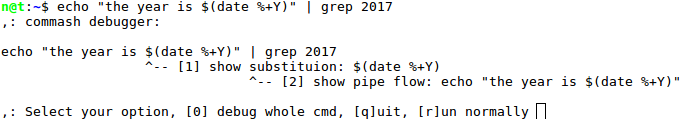
\includegraphics[width=1.0\textwidth]{./images/debugger}
		%\caption{Bash Debugger}
	\end{figure}
\end{frame}



\subsection{Bezpečné příkazy}
\begin{frame}
	\frametitle{Comma-shell: Safe commands}
	
	\begin{exampleblock}{Využití}
		\begin{itemize}
			\item Wrapper základních příkazů
			\item Výpis dalších informací
			\item Změny provedené těmito příkazy lze vrátit zpět
		\end{itemize}
	\end{exampleblock}		
	
	
	\begin{exampleblock}{Implementace}
		\begin{itemize}
			\item Funkce se stejným jménem jako příkaz z GNU coreutils
			\item Logování příkazů a jejich efektů
			\item rm implementováno pomocí FreeDestkop.org koše (trash-cli)
		\end{itemize}
	\end{exampleblock}		
\end{frame}


\begin{frame}
	\frametitle{Ukázka: Comma-shell safe 1/2}
	\begin{figure}
		\centering
		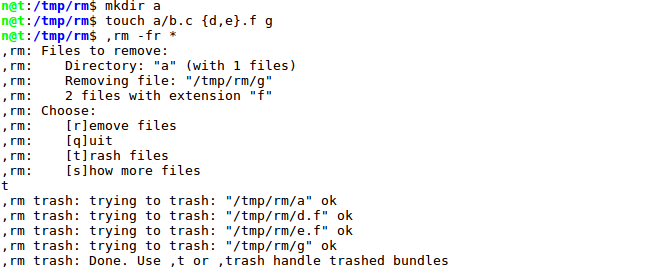
\includegraphics[width=1.0\textwidth]{./images/2rm1}
	\end{figure}
\end{frame}

\begin{frame}
	\frametitle{Ukázka: Comma-shell safe 2/2}
	\begin{figure}
		\centering
		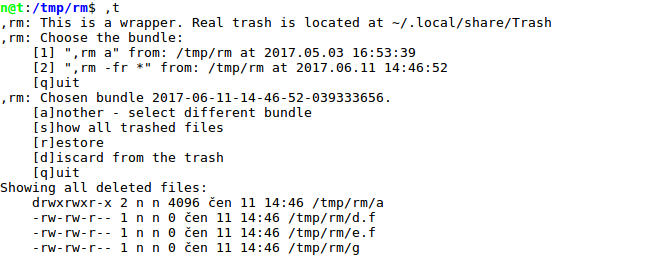
\includegraphics[width=1.0\textwidth]{./images/2rm2}
	\end{figure}
\end{frame}




%\section{Ukázky}




%\section{Instalace}
%\begin{frame}
%	\frametitle{Instalace}
%	
%	\begin{exampleblock}{Git repozitář}
%		\begin{itemize}
%			\item github.com/nesro/commash
%		\end{itemize}
%	\end{exampleblock}
%	
%	
%	\begin{exampleblock}{Instalace}
%		\begin{itemize}
%			\item sudo apt install git shellcheck python-pip xdotool -y
%			\item sudo pip install bashlex
%			\item git clone https://github.com/nesro/commash \textasciitilde/.commash
%			\item source \textasciitilde/.commash/comma.sh
%		\end{itemize}
%	\end{exampleblock}
%\end{frame}

	
%%%%%%%%%%%%%%%%%%%%%%%%%%%%%%%%%%%%%%%%%%%%%%%%%%%%%%%%%%%%%%%%%%%%%%%%%%%%%%%%

%\begin{frame}
%	\frametitle{Děkuji za pozornost}
%	\begin{exampleblock}{Shrnutí}
%		\begin{itemize}
%			\item Formáty COO, CSR, BSR, Quadtree
%			\item Zobecnění formátu Quadtree, husté a řídké listy
%		\end{itemize}
%	\end{exampleblock}
%\end{frame}

%%%%%%%%%%%%%%%%%%%%%%%%%%%%%%%%%%%%%%%%%%%%%%%%%%%%%%%%%%%%%%%%%%%%%%%%%%%%%%%%


%\appendix
\backupbegin


\begin{frame}
	\frametitle{Děkuji za pozornost}
	\begin{exampleblock}{Shrnutí}
		\begin{itemize}
			\item Hooks
			\item Debugger
			\item Safe příkazy
		\end{itemize}
	\end{exampleblock}
\end{frame}

\section{Otázky: oponent}

\begin{frame}
	\frametitle{Otázky: oponent (1/2)}
	\begin{exampleblock}{}
		\begin{itemize}
			\item Comma-shell používá pro vlastní spuštění trasovaných a debugovaných příkazů příkaz eval.
Jak se vypořádá s použitím tohoto příkazu?
		\end{itemize}
	\end{exampleblock}
	\begin{alertblock}{}
	   \begin{itemize}
			\item Příkaz eval je možné spouštět rekurzivně.
			\item Comma-shell příkazem eval spustí více příkazů, ale na rekurzivní spouštění to nemá vliv.
		\end{itemize}
	\end{alertblock}	
\end{frame}

\begin{frame}
	\frametitle{Otázky: oponent (2/2)}
	\begin{exampleblock}{}
		\begin{itemize}
			\item V práci jsem nenašel uživatelskou příručku s výčtem debugovatelných konstrukcí shellu.
Můžete doplnit, které konstrukce Comma-shell podporuje a které ne?
		\end{itemize}
	\end{exampleblock}
	\begin{alertblock}{}
	   \begin{itemize}
			\item Konstrukce, s kterými umí Comma-shell debugger (v interkativním shellu) pracovat jsou: roura, subshell, cykly for a while
			\item Přidání dalších konstrukcí, se kterými umí pracovat knihovna bashlex je snadné
		\end{itemize}
	\end{alertblock}	
\end{frame}


\backupend


\end{document}
